\documentclass[12pt,pdftex]{article}
\usepackage[pdftex]{graphicx,color}
\usepackage{setspace,palatino,multirow}
\usepackage{amsmath,amssymb}
\usepackage{titlesec}
\usepackage{lscape}
%\usepackage{subfigure}
\usepackage{threeparttable}
\usepackage{natbib}
\bibliographystyle{ecta}
\usepackage{cite}
\usepackage{booktabs}
\usepackage{subcaption}
\usepackage{pdflscape}
\usepackage{afterpage}
\usepackage{xcolor}
\usepackage{rotating}
\usepackage[listings, most]{tcolorbox}
\definecolor{nblue}{RGB}{0,0,128}
\usepackage{afterpage}
\usepackage{longtable}

\usepackage[pdftex,colorlinks=true, bookmarks=false,
pdfstartview={XYZ null null 0.85},
pdftitle={Trade in AI-Related Products},
pdfauthor={Michael E. Waugh},
pdfkeywords={tariffs, trade wars, Minneapolis Fed, trade policy
Trade Restrictiveness Index, U.S. trade policy, Deadweight loss},
colorlinks=true,linkcolor=darkgray,citecolor=darkgray,urlcolor=darkgray,
breaklinks]{hyperref}


\newcounter{saveeqni}%
\newcounter{saveeqn01i}%
\newcommand{\alpheqni}{\setcounter{saveeqni}{\value{section}}%
%\setcounter{saveeqn01i}{\value{subsectioni}}%
\renewcommand{\theequation}
    {\alph{saveeqni}\mbox{.\arabic{equation}}}}%
\newcommand{\reseteqni}{\setcounter{equation}{\value{saveeqni}}%
\renewcommand{\theequation}{\arabic{equation}}}%

\newtheorem{as}{Assumption}
\newtheorem{reg}{Regularity Condition}
\newtheorem{conjecture}{Conjecture}
\newtheorem{corr}{Corollary}
\newtheorem{df}{Definition}
\newtheorem{lemma}{Lemma}
\newtheorem{prp}{Proposition}
\newtheorem{rmk}{Remark}
\newenvironment{prf}{{\bf Proof}}{\hfill { }}
\newenvironment{prompt}{\par\medskip\noindent}{\par\medskip}

\DeclareMathOperator*{\plim}{plim}
\DeclareMathOperator*{\umax}{max}

\special{papersize=8.5in,11in}
\onehalfspacing
\setlength{\parindent}{0.1em}
\setlength{\parskip}{.09in}
\textwidth15.75cm
\evensidemargin 1.5in
\oddsidemargin 1.5in
\topmargin 8.5cm
\textheight 10in
\hyphenation{over-lapping}

\tcolorboxenvironment{prp}{%
boxrule = 0mm, breakable, colframe=white,
before skip=5pt,after skip=5pt,
colback=gray!5!white,
top = 2mm,
bottom = 2mm%,
%borderline north={1pt}{1pt}{gray},
%borderline south={1pt}{1pt}{gray}
}

\tcolorboxenvironment{prompt}{%
boxrule = 0mm, breakable, colframe=white,
before skip=5pt,after skip=5pt,
colback=gray!5!white,
top = 2mm,
bottom = 2mm%,
%borderline north={1pt}{1pt}{gray},
%borderline south={1pt}{1pt}{gray}
}

\titleformat{\section}{\color{black}\large\bf}{\color{black}{\thesection.}}{.25cm}{}
\titleformat{\subsection}{\color{black}\normalsize\bf}{\thesubsection.}{.5em}{}
\titleformat{\subsubsection}{\color{black}\normalsize\bf}{\thesubsubsection.}{.5em}{}

\titlespacing{\section}{0pt}{*1.5}{*.5}
\titlespacing{\subsection}{0pt}{*1.5}{*.5}
\titlespacing{\subsubsection}{0pt}{*1.5}{*.5}

\def\thesection{\arabic{section}}
\def\thesubsection{\arabic{section}.\arabic{subsection}}
\def\thesubsubsection{\arabic{section}.\arabic{subsection}.\Alph{subsubsection}}

\def\citeapos#1{\citeauthor{#1}'s (\citeyear{#1})}

\renewcommand{\arraystretch}{1.1}
\usepackage[margin=2cm]{geometry}

\newcommand{\aiRelevantIndex}{204} % AI-relevant imports index (2023=100)
\newcommand{\aggregateIndex}{111} % Aggregate imports index (2023=100)
\newcommand{\notAiRelevantIndex}{96} % Non-AI-relevant imports index (2023=100)
\newcommand{\lastObsDate}{October 2025} % Last observation date
\newcommand{\aiShareTwentyThree}{14} % AI share of total imports in 2023 (%)
\newcommand{\aiShareTwentyFour}{16} % AI share of total imports in 2024 (%)
\newcommand{\aiShareTwentyFive}{21} % AI share of total imports in 2025 (%)
\newcommand{\aiShareGrowth}{7} % AI share growth 2023-2025 (percentage points)
\newcommand{\highAiHsCodes}{612} % Number of HS10 codes classified as high AI relevance
\newcommand{\highAiTwentyThree}{369} % High AI relevance imports in 2023 ($B)
\newcommand{\highAiTwentyFive}{514} % High AI relevance imports in 2025 ($B)
\newcommand{\highAiPctChange}{39} % High AI relevance percent change 2023-2025
\newcommand{\lowAiHsCodes}{15929} % Number of HS10 codes classified as low AI relevance
\newcommand{\lowAiTwentyThree}{1781} % Low AI relevance imports in 2023 ($B)
\newcommand{\lowAiTwentyFive}{1539} % Low AI relevance imports in 2025 ($B)
\newcommand{\lowAiPctChange}{-14} % Low AI relevance percent change 2023-2025
\newcommand{\totalTradeHsCodes}{18364} % Total number of HS10 codes in dataset
\newcommand{\totalTradeTwentyThree}{2598} % Total imports in 2023 ($B)
\newcommand{\totalTradeTwentyFive}{2418} % Total imports in 2025 ($B)
\newcommand{\totalTradePctChange}{-7} % Total trade percent change 2023-2025
\newcommand{\ComputeHardwareHsCodes}{151} % Number of HS10 codes in Compute Hardware
\newcommand{\ComputeHardwareTwentyThree}{144} % Compute Hardware imports in 2023 ($B)
\newcommand{\ComputeHardwareTwentyFive}{274} % Compute Hardware imports in 2025 ($B)
\newcommand{\ComputeHardwarePctChange}{91} % Compute Hardware percent change 2023-2025
\newcommand{\ElectricalPowerHsCodes}{240} % Number of HS10 codes in Electrical Power
\newcommand{\ElectricalPowerTwentyThree}{105} % Electrical Power imports in 2023 ($B)
\newcommand{\ElectricalPowerTwentyFive}{99} % Electrical Power imports in 2025 ($B)
\newcommand{\ElectricalPowerPctChange}{-5} % Electrical Power percent change 2023-2025
\newcommand{\NetworkingTelecomHsCodes}{26} % Number of HS10 codes in Networking Telecom
\newcommand{\NetworkingTelecomTwentyThree}{63} % Networking Telecom imports in 2023 ($B)
\newcommand{\NetworkingTelecomTwentyFive}{80} % Networking Telecom imports in 2025 ($B)
\newcommand{\NetworkingTelecomPctChange}{26} % Networking Telecom percent change 2023-2025
\newcommand{\CoolingHVACHsCodes}{134} % Number of HS10 codes in Cooling HVAC
\newcommand{\CoolingHVACTwentyThree}{39} % Cooling HVAC imports in 2023 ($B)
\newcommand{\CoolingHVACTwentyFive}{39} % Cooling HVAC imports in 2025 ($B)
\newcommand{\CoolingHVACPctChange}{-1} % Cooling HVAC percent change 2023-2025
\newcommand{\BuildingStructureHsCodes}{29} % Number of HS10 codes in Building Structure
\newcommand{\BuildingStructureTwentyThree}{9} % Building Structure imports in 2023 ($B)
\newcommand{\BuildingStructureTwentyFive}{7} % Building Structure imports in 2025 ($B)
\newcommand{\BuildingStructurePctChange}{-27} % Building Structure percent change 2023-2025
\newcommand{\SpecialtyMaterialsHsCodes}{22} % Number of HS10 codes in Specialty Materials
\newcommand{\SpecialtyMaterialsTwentyThree}{7} % Specialty Materials imports in 2023 ($B)
\newcommand{\SpecialtyMaterialsTwentyFive}{14} % Specialty Materials imports in 2025 ($B)
\newcommand{\SpecialtyMaterialsPctChange}{98} % Specialty Materials percent change 2023-2025
\newcommand{\FireSafetySecurityHsCodes}{9} % Number of HS10 codes in Fire Safety Security
\newcommand{\FireSafetySecurityTwentyThree}{1} % Fire Safety Security imports in 2023 ($B)
\newcommand{\FireSafetySecurityTwentyFive}{1} % Fire Safety Security imports in 2025 ($B)
\newcommand{\FireSafetySecurityPctChange}{-5} % Fire Safety Security percent change 2023-2025
\newcommand{\totalHighAiHsCodes}{612} % Total HS10 codes across all high AI categories
\newcommand{\totalHighAiTwentyThree}{369} % Total high AI imports in 2023 ($B)
\newcommand{\totalHighAiTwentyFive}{514} % Total high AI imports in 2025 ($B)
\newcommand{\totalHighAiPctChange}{39} % Total high AI percent change 2023-2025
\newcommand{\tariffHighTwentyFour}{1.8} % High AI relevance tariff rate in 2024 (%)
\newcommand{\tariffHighTwentyFive}{4.6} % High AI relevance tariff rate in 2025 (%)
\newcommand{\tariffLowTwentyFour}{2.7} % Low AI relevance tariff rate in 2024 (%)
\newcommand{\tariffLowTwentyFive}{9.1} % Low AI relevance tariff rate in 2025 (%)
\newcommand{\tariffComputeHardwareTwentyFour}{0.5} % Compute Hardware tariff rate in 2024 (%)
\newcommand{\tariffComputeHardwareTwentyFive}{1.2} % Compute Hardware tariff rate in 2025 (%)
\newcommand{\tariffElectricalPowerTwentyFour}{3.8} % Electrical Power tariff rate in 2024 (%)
\newcommand{\tariffElectricalPowerTwentyFive}{11.8} % Electrical Power tariff rate in 2025 (%)
\newcommand{\tariffNetworkingTelecomTwentyFour}{1.5} % Networking Telecom tariff rate in 2024 (%)
\newcommand{\tariffNetworkingTelecomTwentyFive}{4.1} % Networking Telecom tariff rate in 2025 (%)
\newcommand{\tariffCoolingHVACTwentyFour}{2.9} % Cooling HVAC tariff rate in 2024 (%)
\newcommand{\tariffCoolingHVACTwentyFive}{10.3} % Cooling HVAC tariff rate in 2025 (%)


\begin{document}


\begin{onehalfspacing}

{\large \textbf{Trade in AI-Related Products}}

\vspace{0.5cm}

\href{http://www.waugheconomics.com/}{Michael E. Waugh} \\ Federal Reserve Bank of Minneapolis and NBER

\vspace{0.5cm}

February 2026

\vspace{0.5cm}



\vspace{1.5cm}


\normalsize

ABSTRACT ------------------------------------------------------------------------------------------------------------

This paper documents facts about international trade in AI-related products. I develop a large language model (LLM) classification tool that maps HS10 codes in U.S. trade data to inputs used in the construction and operation of AI infrastructure. AI-related products account for 23 percent of U.S. imports in 2025, and these products have grown by \highAiPctChange{} percent since 2023. Over this same time period, non-AI-related products have grown by only \lowAiPctChange{} percent with the divergence between the two categories beginning in early 2024. U.S. exports of AI-related products have been similarly strong, suggestive that U.S. exporters play an important role in the AI global value chain. Mexico is a key market for both the import and export side, and along with Taiwan these two countries accounting for about half of all AI trade. AI-related products face lower tariffs, \tariffHighTwentyFive{} percent versus \tariffLowTwentyFive{} percent for non-AI-related products. These facts point to an important source of resilience in U.S. trade since the re-emergence of protectionism in 2025. 

------------------------------------------------------------------------------------------------------------------------------
\vspace{0.25cm}

JEL Classification: F13, F14\\
%%
%%
Keywords: Tariffs, U.S. Trade Policy, Trade Restrictiveness Index

% need to run notebooks: TRI-all-country.ipynb
% then run TRI-sector

\vspace{3.0cm}

{\footnotesize Email: michael.e.waugh@gmail.com. The views expressed herein are those of the author and not necessarily those of the Federal Reserve Bank of Minneapolis or the Federal Reserve System. My github repository provides the code and supplementary work behind this paper at \url{https://github.com/}.}

\hspace{-0.05cm}

\newpage

The United States is experiencing a massive AI-investment driven boom with hundreds of billions, if not trillions, of dollars being invested in the build out of datacenters and other related AI-infrastructure projects. This paper asks the question: How is this AI-datacenter build out influencing international trade flows? The answer is that trade in AI-related products is perhaps \emph{the} dominant force in U.S. trade flows over the past two years. And this observation is despite the dramatic changes in U.S. trade policy that have taken place over this time period. 

Key to answering this question requires some knowledge about what products are related to AI-infrastructure. My approach uses a large language model (LLM) classification tool that maps knowledge and descriptions of products available in trade data into a systematic classification of if that product might be used in AI-infrastructure and how it is used. This classification allows me to take unstructured descriptions and then construct structured measures of international trade in AI-related products.

What are AI-related products? My classification tool identifies the unusual suspects like data processing units, storage devices, etc. These computer hardware components account for half of all AI-related products and imports of these products have grown by triple digits since 2023. However, my classification tool also identifies a broader array of products that relate to electrical infrastructure, networking, cooling and HVAC, and specialty materials. These ancillary products account for the other half of AI-related products and have displayed double digit import growth.  

In aggregate, these AI-related products are a dominant force behind U.S trade flows. Through 2025, they account for nearly a quarter of all U.S. imports. And this share was half as small in 2023. Leading into 2023, AI-related products grew no differently than non-AI-related products. But since early 2024, import growth in AI-related products exploded | see Figure \ref{fig:ai-trade-index}. Exports of AI-related products display a similar trend and the destinations and products suggests that trade in AI-related products is not onesided, but that U.S. exporters play an important role in the AI global value chain.

Two countries play an important role in the sourcing of AI-related products. Not surprisingly, Taiwan is an important source for computer hardware components (e.g. semiconductors) and Taiwan accounts for about a quarter of imports of AI-related products. The surprising source is Mexico. They account for another quarter of AI-related trade and their reach is important in computer hardware and other products related to electrical power, networking, and cooling HVAC. 

 





%https://www.bloomberg.com/news/articles/2026-02-06/how-much-is-big-tech-spending-on-ai-computing-a-staggering-650-billion-in-2026
%
%https://www.axios.com/2026/02/06/amazon-microsoft-meta-ai-investment
%
%the GDP contribution depends on how much imported content there is .

%https://www.wsj.com/tech/ai/ai-spending-tech-companies-compared-02b90046?mod=livecoverage_web

%https://www.goldmansachs.com/insights/articles/why-ai-companies-may-invest-more-than-500-billion-in-2026

%Goldman Sachs
%2026 projections ($527B hyperscaler capex, $1.15T for 2025-2027):
%https://www.goldmansachs.com/insights/articles/why-ai-companies-may-invest-more-than-500-billion-in-2026

%$1 trillion investment by 2027, $5 trillion for infrastructure:
%https://pwm.gs.com/nam/en-us/insights/markets-and-investing/innovation-technology/the-building-blocks-behind-ai-next-wave

%$1.4 trillion for 2025-2027 (includes breakdown by company):
%https://www.goldmansachs.com/what-we-do/investment-banking/insights/articles/powering-the-ai-era/report.pdf

%$200 billion globally by 2025 (earlier 2023 estimate):
%https://www.goldmansachs.com/insights/articles/ai-investment-forecast-to-approach-200-billion-globally-by-2025
%Technology sector outlook with capex estimates:

%https://am.gs.com/en-ae/advisors/insights/article/2025/technology-in-2025-the-cycle-rolls-on

%S&P Global
%$61 billion data center deals in 2025, $600B 2026 hyperscaler capex:
%https://www.cnbc.com/2025/12/19/data-center-deals-hit-record-amid-ai-funding-concerns-grip-investors.html
%80% of US private demand growth from AI infrastructure:
%https://www.spglobal.com/en/research-insights/special-reports/look-forward/data-center-investment-moves-macro-needle
%~40% increase to $600B in 2026:
%https://www.ciodive.com/news/ai-boost-cloud-spending/810399/
%$450 billion in transactions over 5 years:
%https://www.spglobal.com/en/research-insights/special-reports/look-forward/data-center-frontiers/data-center-risk-if-ai-promises-fade
%McKinsey & Company
%$6.7 trillion total, $5.2 trillion for AI infrastructure by 2030:
%https://www.mckinsey.com/industries/technology-media-and-telecommunications/our-insights/the-cost-of-compute-a-7-trillion-dollar-race-to-scale-data-centers
%Bloomberg/Major Financial Press
%$3 trillion total buildout, recent company guidance:
%https://www.bloomberg.com/news/articles/2026-02-02/the-3-trillion-ai-data-center-build-out-spurs-a-debt-market-boom
%$600B+ for 2026 (Big Five hyperscalers):
%https://techblog.comsoc.org/2025/12/22/hyperscaler-capex-600-bn-in-2026-a-36-increase-over-2025-while-global-spending-on-cloud-infrastructure-services-skyrockets/
%$650 billion 2026 estimate (Amazon $200B, Alphabet $175-185B, etc.):
%https://finance.yahoo.com/news/big-tech-set-to-spend-650-billion-in-2026-as-ai-investments-soar-163907630.html
%Big Tech $380 billion spending in 2025:
%https://www.cnbc.com/2025/12/24/ai-infrastructure-stocks-lumentum-celestica-seagate-beat-nvidia-2025.html
%Additional High-Quality Sources
%KKR analysis ($7 trillion McKinsey estimate cited):
%https://www.kkr.com/insights/ai-infrastructure
%JLL global data center report ($3 trillion over 5 years):
%https://www.jll.com/en-us/newsroom/global-data-center-sector-to-nearly-double-to-200gw-amid-ai-infrastructure-boom
%PBS NewsHour interview with NYT reporter on AI spending:
%https://www.pbs.org/newshour/show/whats-next-for-ai-and-has-its-explosive-growth-in-2025-created-a-bubble


\section{Classifying AI-Related Products}\label{sec:measurment}

This section describes how I classify internationally traded commodities that are plausibly used to build and operate AI-focused data centers | hyperscale facilities that rely on GPU servers, high-speed networking, and high-density power and cooling. The measurement question is: which traded goods plausibly enter AI data-center construction, equipping, and operations?

I treat this as a classification problem and use a large language model (LLM) to systematically label the universe of HS10 commodity codes (about 19,000) by their relevance to AI data-center infrastructure. There are many examples of using LLMs for classification purposes in economics. For example, \citet{clayton2025geoeconomic} develop measures of ``geoeconomic pressure'' by using an LLM to read earnings calls and classify which governments apply pressure, to whom, and how. Similarly, \citet{lagakos2025american} use LLMs to extract systematic information from individuals' life narratives on sources of meaning and overall life satisfaction. The methodological idea is the same | provide the LLM a list of commodity descriptions and then ask systematic questions about the relevance of the product to AI infrastructure.

\subsection{Data}

Several inputs are provided to the LLM. First, I use a list of 10-digit Harmonized System commodity codes from U.S. Census Bureau trade statistics. The HS10 classification provides the finest level of product disaggregation available in U.S. trade data, with \totalTradeHsCodes{} distinct codes found 2024 import and export data. Each HS10 code includes a standardized commodity description. As an example, consider
\begin{prompt}
\noindent\texttt{8542310040: PROCESSORS (INCLUDING MICROPROCESSORS): GRAPHICS PROCESSING UNITS (GPUS).}
\end{prompt}
where \texttt{8542310040} is the HS10 code and the description indicates that this product is a processor and specifically a GPU. This is a canonical \textbf{High} example. 

The second input that I provide to the LLM is the 6-digit NAICS classification code and the associated description that relates to the HS10 code above. The idea here is to provide the LLM with more context about the HS10 code. NAICS codes do so because they are production oriented, and thus provide context about how the product may be used. I use the concordance provided by the \href{https://www.census.gov/foreign-trade/schedules/b/2022/imp-code.txt}{Census} which provides a mapping from HS10 codes to the six digit NAICS codes. In cases where there are multiple NAICS associated with an HS10 code, I provide the LLM with a list of the NAICS codes and associated descriptions. 

Finally, I restrict attention only to commodities that do not include petroleum products, precious metals, or HS2 chapters 98 and 99 which include art, antiques, and other special provisions. 

\subsection{LLM Classification Procedure}

The classification procedure requires specifying both a categorization scheme and a prompt to implement it. The primary scheme that I implement is to classify each HS10 code into one of three bins:
\begin{itemize}
    \item \textbf{High}: Products directly used in data center construction or operation, with clear application to compute, cooling, power, networking, or facility infrastructure
    \item \textbf{Medium}: Products with plausible data center applications but also significant non-data-center uses, or indirect inputs to data center materials
    \item \textbf{Low}: Products with no apparent connection to data center construction
\end{itemize}
In the baseline results, I focus on products classified as \textbf{High}. I only treat \textbf{Medium}-rated products for robustness considerations.

In addition to this categorization, I also ask the model to provide a confidence score, a use category, and finally, a natural language explanation of the classification decision. These additional outputs provide the ability to ex-post scrutinize the classification. So, for each HS10 code $i$ with description $d_i$, I prompt the model to return a structured classification object:
\begin{align*}
    C_i = \{\texttt{relevance}_i, \ \texttt{confidence}_i, \ \texttt{category}_i, \ \texttt{reasoning}_i\}
\end{align*}
\noindent where:
\begin{itemize}
    \item $\texttt{relevance}_i \in \{\text{\textbf{High}}, \text{\textbf{Medium}}, \text{\textbf{Low}}\}$ is constrained by an enumerated type,
    \item $\texttt{confidence}_i \in [0, 100]$ is an integer confidence score,
    \item $\texttt{category}_i$ maps to one of eight predefined categories (Compute Hardware, Networking/Telecom, Cooling/HVAC, Electrical/Power, Building Structure, Fire Safety/Security, Specialty Materials, Not DC Related),
    \item $\texttt{reasoning}_i$ provides a natural language explanation of the classification decision.
\end{itemize}
The schema enforcement ensures that every response contains valid values for all fields. The model cannot return ``Medium-High'' or ``Moderate'', etc. It will only return the three specified relevance levels. The structured approach also facilitates systematic analysis and the comparison of outputs across different LLM models.

An important input is the prompt to the LLM. The prompt provides context on AI data center construction and describes the categories of relevant products. The prompt also ensures that the output is structured according to the schema described above. The complete prompt is presented in the appendix, but the first snippet is the following:
\begin{prompt}
\texttt{You are an expert in AI data center construction, operations, and supply chains. Your task is to classify products by their relevance to building and operating AI-focused data centers (hyperscale facilities running GPU clusters for training and inference. You will be provided with two pieces of information about each product:}\\

\texttt{1. **HS10 Code and Description**: The Harmonized System (HS) is an international product classification used for trade statistics. The HS10 code is a 10-digit code used by U.S. Customs to classify imported goods. The description tells you what the physical product is.}\\

\texttt{2. **NAICS Code and Description**: The North American Industry Classification System (NAICS) indicates which U.S. industry produces or uses this product. This provides additional context about the product's typical industrial application.}\\

\texttt{Consider these categories of relevant products: COMPUTE: GPUs, CPUs, memory, PCBs, servers, storage drives, semiconductors; NETWORKING: Fiber optics, switches, routers, transceivers, cables; COOLING: Chillers, cooling towers, CRAH units, fans, pumps, refrigerants; ELECTRICAL: Transformers, switchgear, UPS, batteries, generators, cables; BUILDING: Structural steel, concrete, rebar, insulation, raised floors; SPECIALTY MATERIALS: Rare earths, copper, aluminum, tantalum, thermal interface materials...}
\end{prompt}
In addition to this prompt, it also instructs the model to consider edge cases explicitly. For example, products like diesel engines could be relevant (for generators) or irrelevant (for vehicles), and that context from the HS code description should guide the determination.

I employ Claude (Anthropic) as my main classification model, using the tool-calling API to obtain structured responses.\footnote{I use the \texttt{claude-sonnet-4-20250514} model. Results are robust to using alternative frontier models; see Appendix \ref{appendix}.} I set the temperature... I process all \totalTradeHsCodes{} HS10 codes through the classification API with rate limiting to respect API constraints. Processing all codes required about a day and a half at a total cost of approximately \$150.

\afterpage{%
\clearpage
%\refstepcounter{table}
\begin{table}[htbp]
\centering
\caption{U.S. Import Values by AI Relevance and Category (2023 vs 2025)}
\label{tab:trade_hierarchical}
\setlength{\tabcolsep}{4.5mm}
\renewcommand{\arraystretch}{1.60}
\begin{tabular}{lrrrr}
\toprule
Category & \# HS10 Codes & 2023 (\$B) & 2025 (\$B) & Change (\%) \\
\midrule
High AI Relevance & 612 & 368.7 & 643.0 & +74.4 \\
\quad\quad Compute Hardware & 151 & 143.8 & 353.5 & +145.8 \\
\quad\quad Electrical Power & 240 & 104.8 & 118.0 & +12.6 \\
\quad\quad Networking Telecom & 26 & 63.3 & 99.8 & +57.7 \\
\quad\quad Cooling HVAC & 134 & 39.3 & 45.5 & +16.0 \\
\quad\quad Building Structure & 29 & 9.2 & 7.6 & -16.4 \\
\quad\quad Specialty Materials & 22 & 7.3 & 17.3 & +136.8 \\
\quad\quad Fire Safety Security & 9 & 1.0 & 1.1 & +9.3 \\
Low AI Relevance & 15929 & 1780.7 & 1810.6 & +1.7 \\
\midrule
Total Trade & 18364 & 2598.3 & 2883.9 & +11.0 \\
\bottomrule
\end{tabular}
\end{table}

}

\section{Facts about AI-Related Trade}\label{sec:facts}

This section discusses several facts that arise from the classification scheme. I proceed in the following steps. First, I discuss what types of products actually show up in the classification schema. Second, I show how these AI-related products have grown substantially since early 2024. Finally, I discuss how AI trade has interacted with the start of the 2025 trade war. 

\subsection{What are AI-Related products?}\label{sec:facts-ai-products}

Table \ref{tab:trade_hierarchical} provides an overview of what the classification scheme identifies. The first row reports all HS10 codes that are classified as \textbf{High} relevance. High relevance codes encompass \totalHighAiHsCodes{} codes out of a total of \totalTradeHsCodes{} codes. The \textbf{High} relevance codes accounted for \aiShareTwentyThree{} percent of total imports in 2023, and this increased to \aiShareTwentyFive{} percent in 2025.

The next seven rows of Table \ref{tab:trade_hierarchical} break down those HS10 codes classified as \textbf{High} into the seven predefined categories discussed above. Amongst those categories, there are essentially four that stand out: Compute Hardware, Electrical Power, Network and Telecom, and then Cooling HVAC. These four categories represent nearly 95 percent of all goods classified as \textbf{High} goods.

Table \ref{tab:top10_high_relevance_landscape} (at the back of the paper) provides further detail into the specific products behind the classification. It reports the top ten HS10 codes in terms of 2025 import volume which were classified as \textbf{High}. For each code, the table reports the Census's short description, the LLM category, the LLM reasoning behind the classification, and various trade statistics.\footnote{The trade statistics are 2025 imports, the share of those imports in total trade, and the change in import volume relative to 2023. The description is the Census short description; this is different from their long description which is what is fed into the LLM.} The dominant HS10 code is {\tt 8471500150} which is described as data processing units. And the LLM reasoned that data processing units are a core component of compute hardware.

While this top 10 list is dominated by other types of computer hardware and networking equipment, there are other products classified as important. In particular, {\tt 7403110000} (refined copper cathodes) is the sixth most important product. The LLM reasoning is that refined copper cathodes are a key input into copper products (e.g., electrical wire) used in data centers. Table \ref{tab:top11to20_high_relevance_landscape} in the appendix reports the next 10 products. 

In looking through Table \ref{tab:trade_hierarchical} or \ref{tab:top10_high_relevance_landscape}, one cannot help but notice the dramatic growth in trade volumes in nearly all categories. The next section discusses this growth.

\subsection{The Spectacular Growth of AI-Related Trade}\label{sec:facts-growth}

Figure \ref{fig:ai-trade-index} is the most important figure in this paper. It plots several different indices of trade volumes. These indices are computed by taking trade volumes in a category for a given month, then normalizing them by the monthly average for 2023. 

 \begin{figure}[t]
\centering
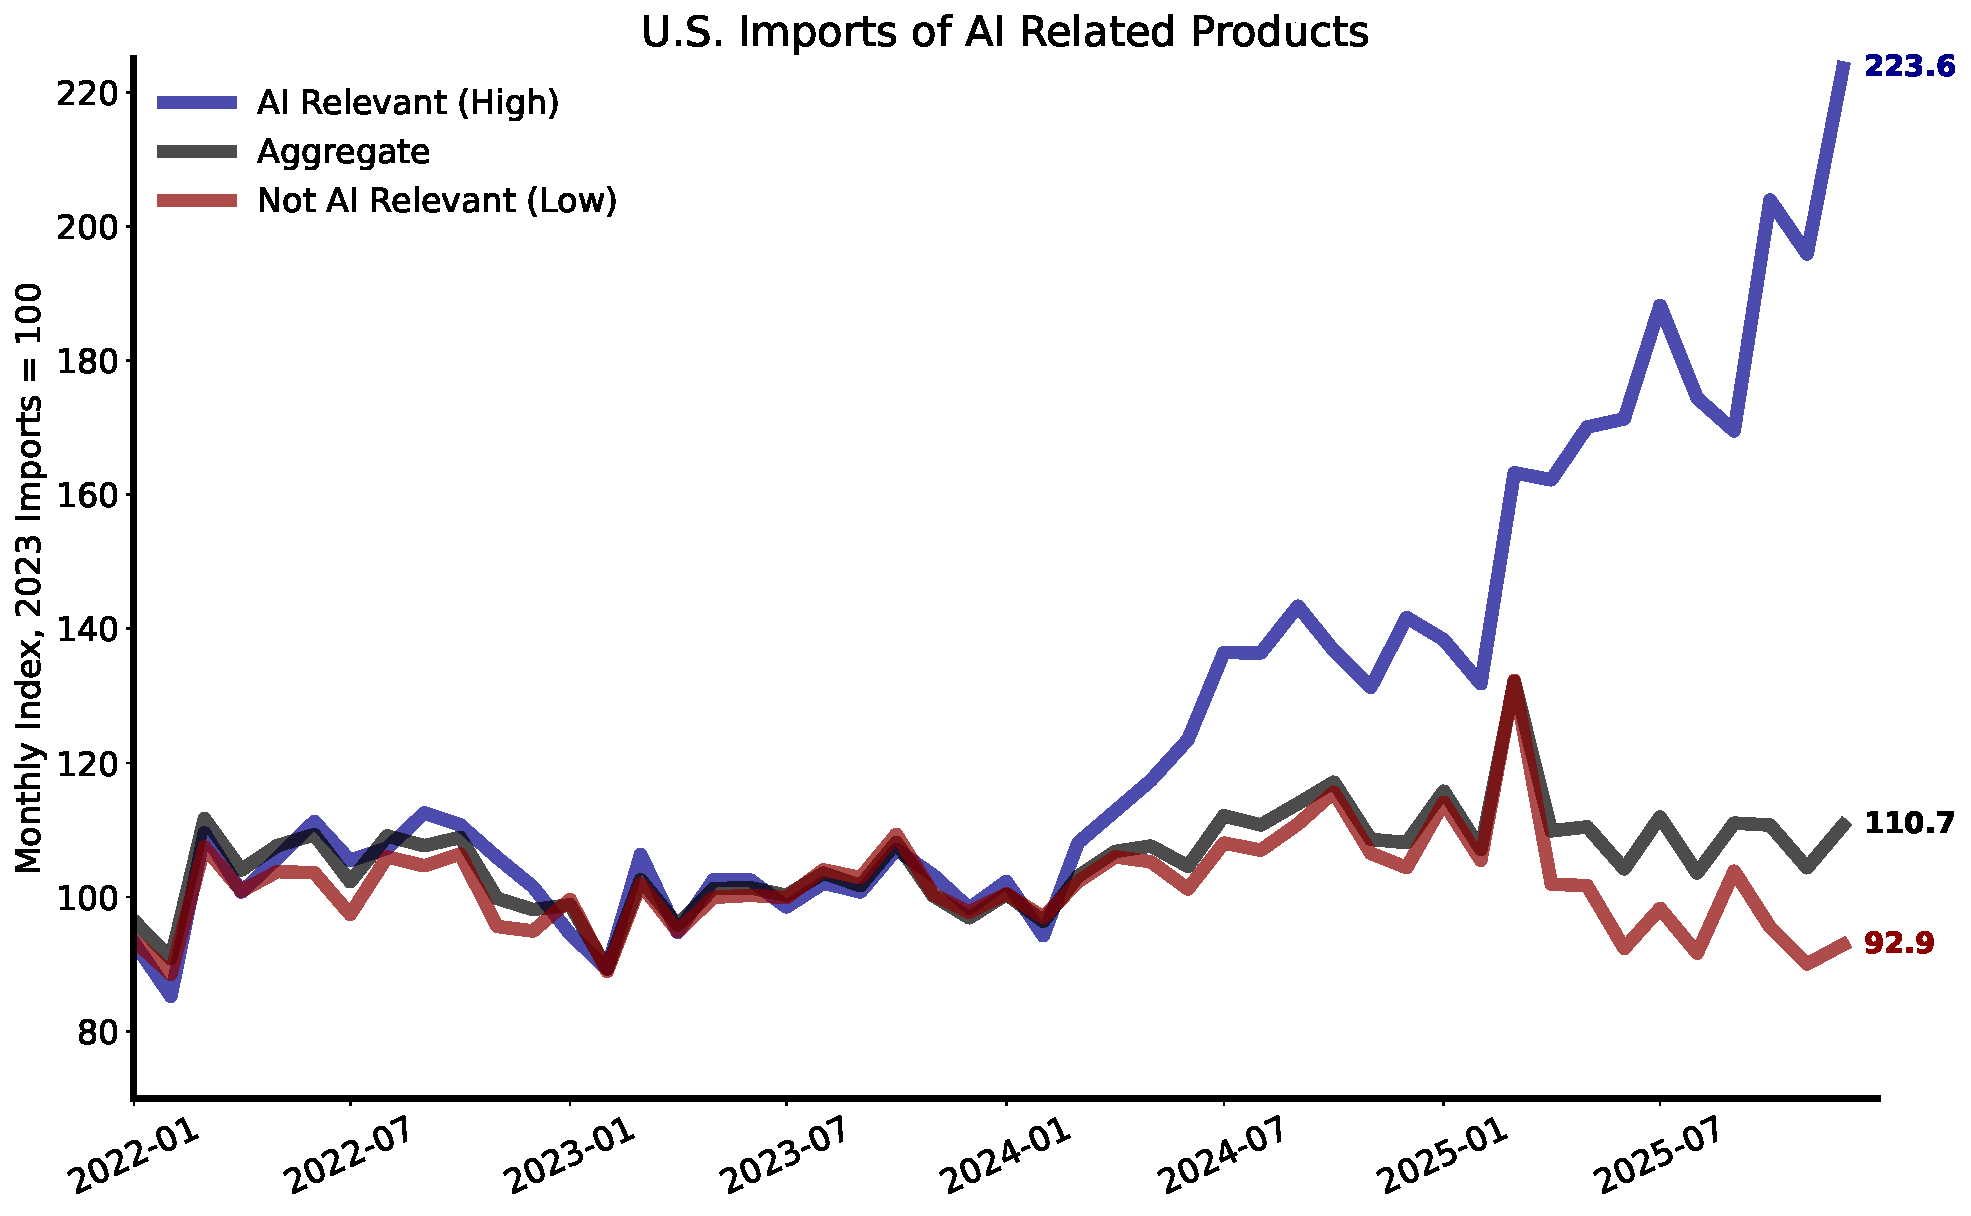
\includegraphics[height=0.45\textheight]{./figures/ai-trade-index.pdf}
\caption{U.S. imports of AI and non-AI products}\label{fig:ai-trade-index}
\end{figure}

Focus on the blue line titled ``AI Relevant.'' This is the index computed for all \textbf{High} products. The most obvious feature of AI-related products is the spectacular growth. Currently, in December of 2025, the index for AI relevant products is \aiRelevantIndex{}, meaning import volumes are 124 percent larger than the typical month in 2023. 

The second observation concerns the timing of the growth. From 2022 to early 2024, there is no differential trend in AI-relevant products relative to non-AI-relevant products. After early 2024, there is divergence and this divergence accelerates in 2025. As a sanity check, this is consistent with the broad narratives about the timing of the AI investment boom. 

Where is the growth coming from? Return to the final column of Table \ref{tab:trade_hierarchical}. For each category, the final column reports 2025 trade volumes relative to 2023 in percent terms. Consistent with Figure \ref{fig:ai-trade-index}, \textbf{High} AI relevant products grew by \highAiPctChange{} percent. Then the breakdown by category shows that this growth is broad-based | there is double digit growth in 5 out of the 7 categories. Focusing on products, Table \ref{tab:top10_high_relevance_landscape} confirms how broad and spectacular the growth is with all of the top 10 HS10 codes displaying double-digit growth; five display triple-digit growth rates. 

 \begin{figure}[t]
\centering
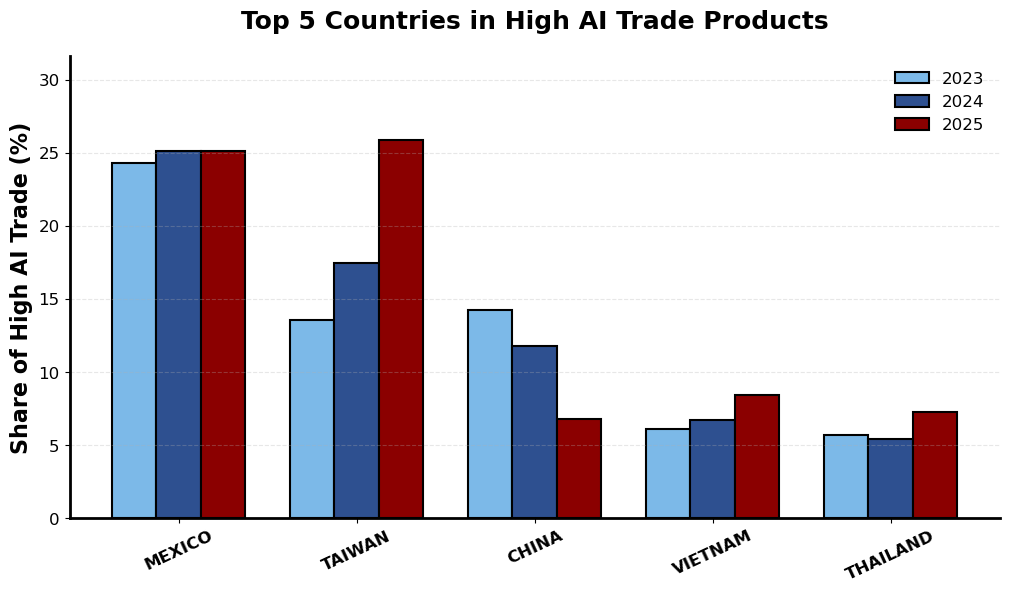
\includegraphics[height=0.40\textheight]{./figures/ai-by-country.png}
\caption{Top Sources of AI Related Products}\label{fig:ai-trade-country}
\end{figure}

The black and red lines report aggregate trade and ``not AI Relevant.'' The latter series is the index computed for all \textbf{Low} products. In aggregate, trade has grown in 2025 by \totalTradePctChange{} percent relative to 2023. This aggregate growth is very strong given that U.S. tariffs increased by more than ten percentage points in 2025. However, this modest growth is simply a byproduct of the spectacular growth in AI-relevant products. Once these products are stripped out, non-AI-relevant imports as of December 2025 are 8 percent below the typical month in 2023. On a year-over-year basis, Table \ref{tab:trade_hierarchical} reports that non-AI-relevant products grew by \lowAiPctChange{} percent and much of this growth owes to the front-running of tariffs in early 2025. 

\subsection{Mexico and Taiwan are Dominant Sources}\label{sec:facts-source}

Where are these products coming from? Figure \ref{fig:ai-trade-country} provides a first look at this by computing the share of \textbf{High} products by source country for each year since 2023. 

Mexico's dominance is a perhaps surprising feature of Figure \ref{fig:ai-trade-country}. Consistently, it has accounted for about 25 percent of \textbf{High} AI-relevant products trade across all years. Less surprising is the role of Taiwan. It is well known that Taiwan is an important source of semiconductor and computer hardware products. Consistent with this notion, Figure \ref{fig:ai-trade-country} shows that Taiwan is important and increasingly dominant in 2025, rivaling Mexico. 

Mexico's role in AI-related trade helps explain some puzzling features of commerce within the USMCA. Both Canada and Mexico had the essentially had the same tariff treatment over the course of 2025. Yet, U.S. imports from Canada have changed by \canadaTotalImportGrowthTwentyFiveVsTwentyFour{} percent whereas U.S. imports from Mexico rose by \mexicoTotalImportGrowthTwentyFiveVsTwentyFour{} percent. Part of this divergence reflects the \mexicoHighAiImportGrowthTwentyFiveVsTwentyFour{} percent growth in Mexican AI-related exports to the U.S.

China has declined in importance. In 2023 it held a similar position to Taiwan, but it has since fallen to a level comparable to Vietnam and Thailand, the fourth and fifth largest sources. 

\begin{figure}[t]
\centering
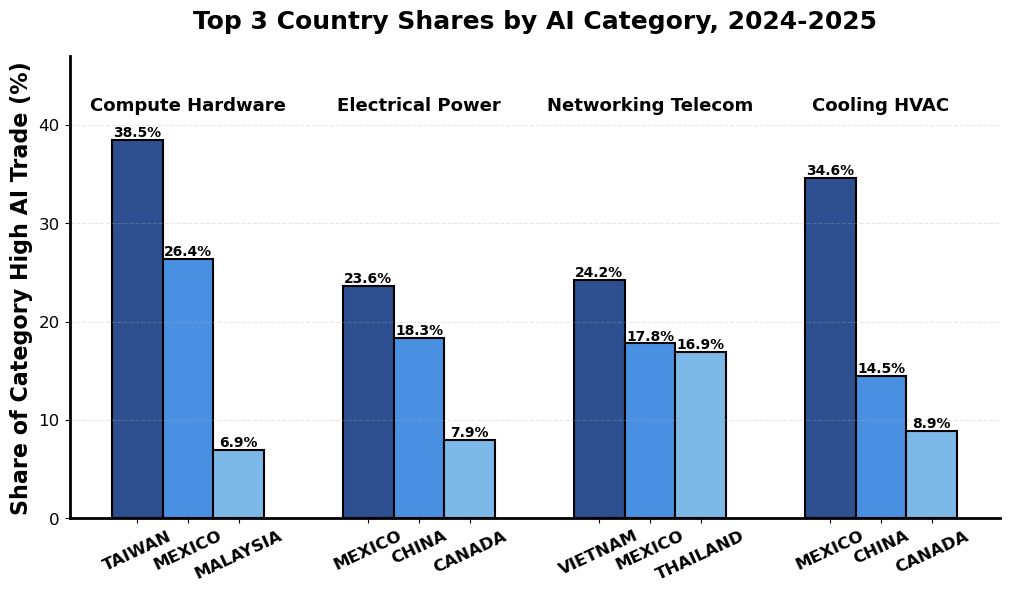
\includegraphics[height=0.40\textheight]{./figures/ai-by-country-category.png}
\caption{Top Sources by AI Related Product Category}\label{fig:ai-trade-country-catagoy}
\end{figure}

Figure \ref{fig:ai-trade-country-catagoy} breaks down the country composition by top categories of AI-related products. In two out of the top four categories, Mexico is the leader in two of the top four categories and ranks second place in every other category. Taiwan's prominence is concentrated in Compute Hardware, where it is the leading source. 
\subsection{Tariffs are lower on AI-Related Products}\label{sec:facts-tariffs}


\begin{figure}[t]
\centering
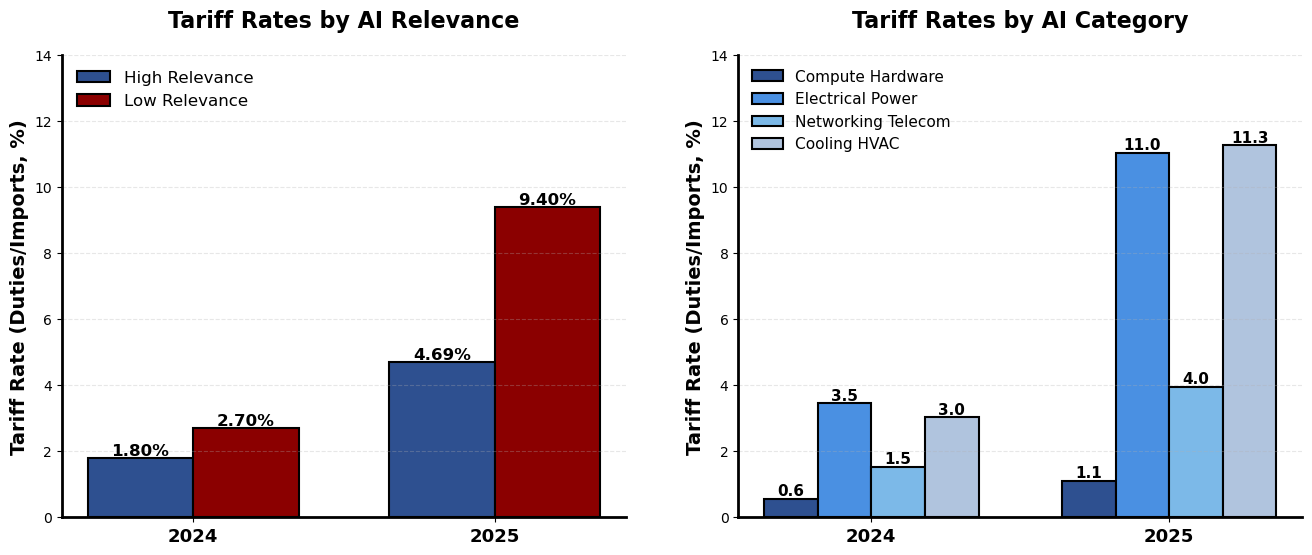
\includegraphics[height=0.30\textheight]{./figures/ai-tariffs.png}
\caption{Tariff Rates on AI and non-AI products}\label{fig:ai-tariffs}
\end{figure}



%\begin{figure}[t]
%\centering
%\caption{Data and Model}\label{fig:simmulated-trade-flows}
%\begin{subfigure}[t]{0.48\textwidth}
%    \centering
%    \caption{Trade Data vs. Exact EK}
%    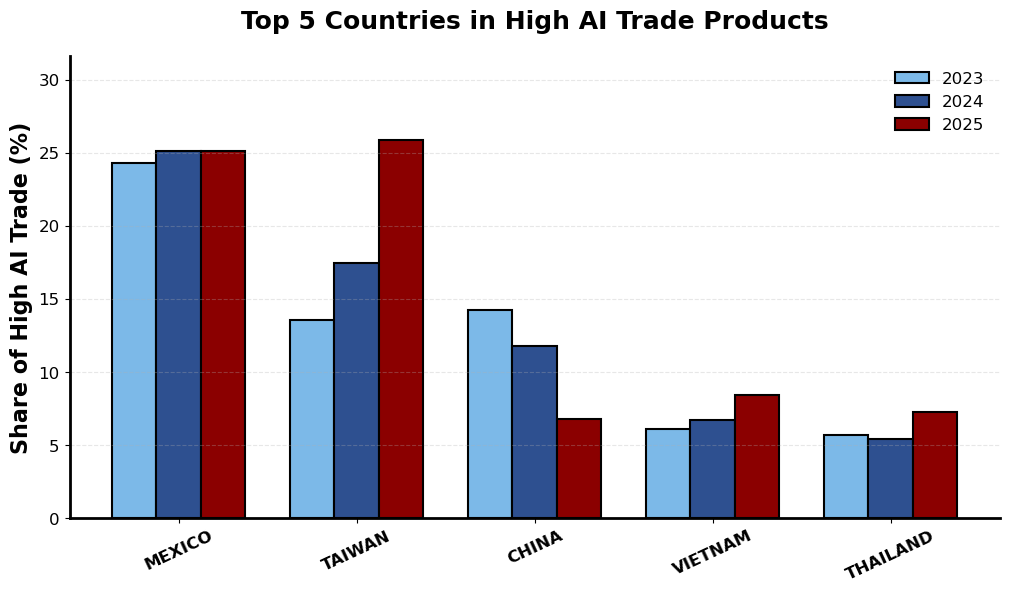
\includegraphics[width=\textwidth]{./figures/ai-by-country.png}
%    \label{fig:trade-flows-exact}
%\end{subfigure}
%\hfill
%\begin{subfigure}[t]{0.48\textwidth}
%    \centering
%    \caption{Exact EK vs. Monte Carlo EK}
%    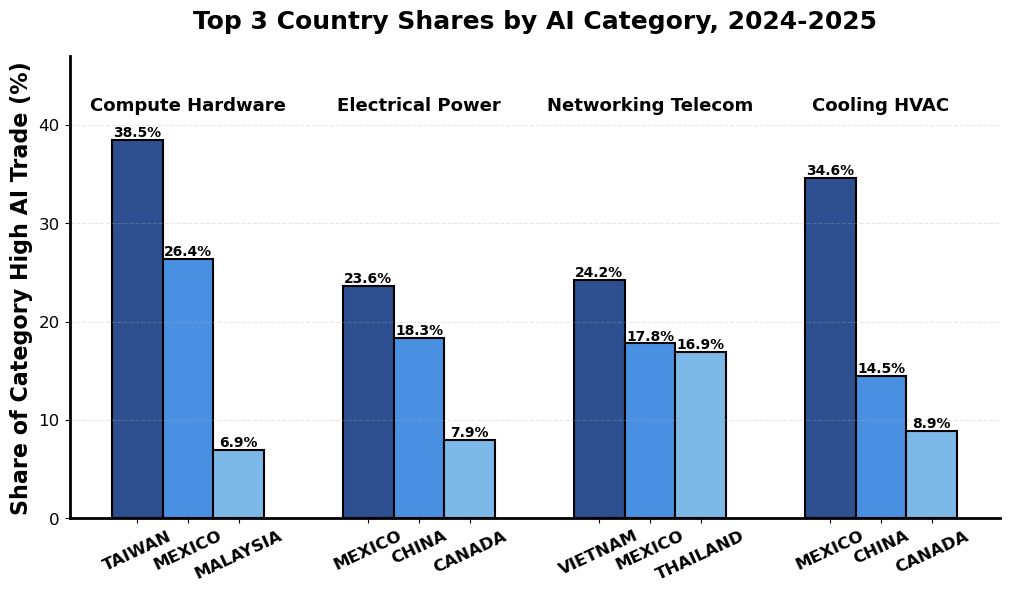
\includegraphics[width=\textwidth]{./figures/ai-by-country-category.png}
%    \label{fig:trade-flows-monte-carlo}
%\end{subfigure}
%\end{figure}


%\afterpage{%
%\clearpage
%\begin{landscape}
%\begin{figure}
%\centering
%\caption{U.S. imports of AI and non-AI products}\label{fig:ai-trade-index}
%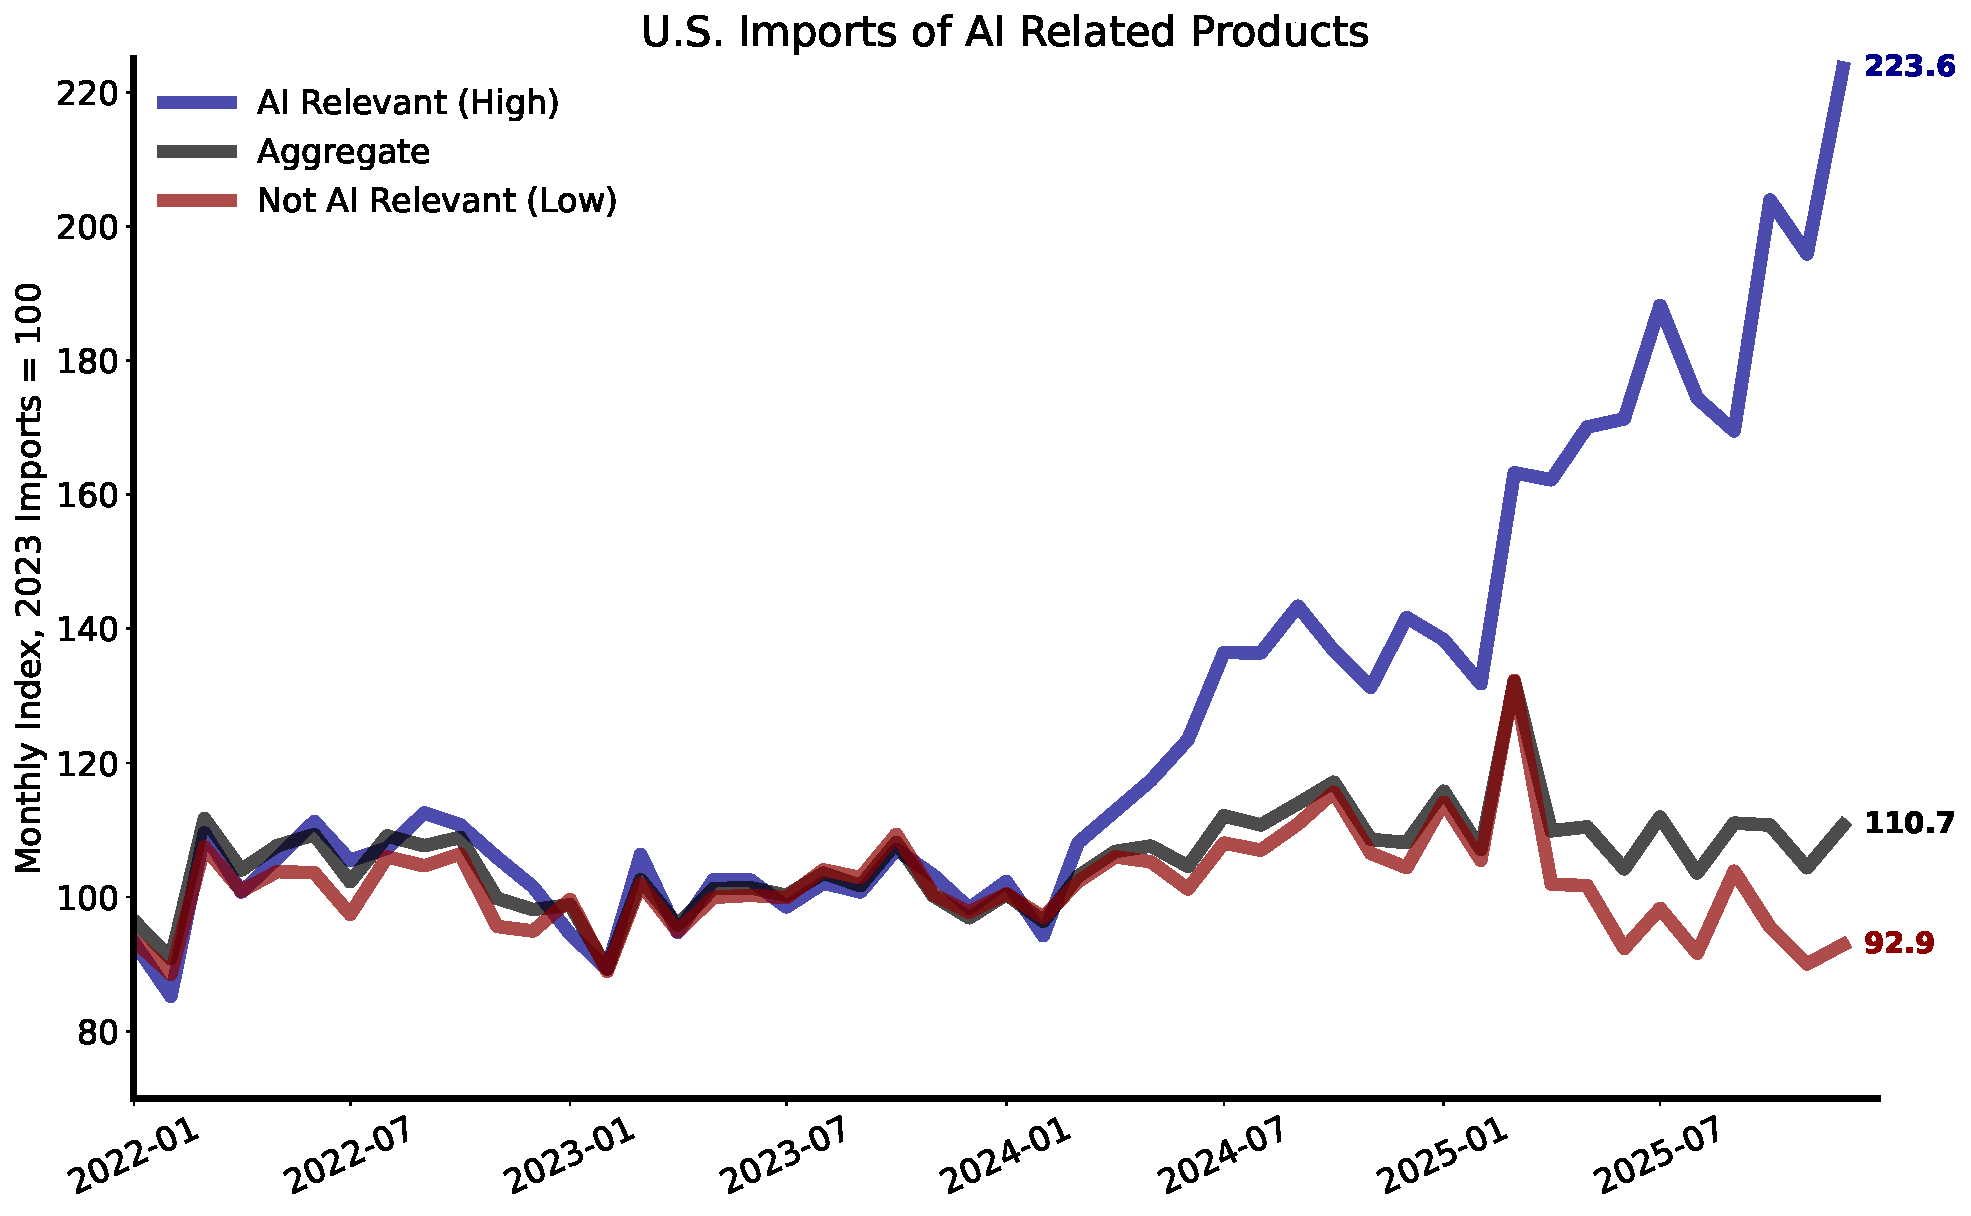
\includegraphics[height=0.80\textheight]{./figures/ai-trade-index.pdf}
%\end{figure}
%\end{landscape}}




%\afterpage{%
%\clearpage
%\begin{landscape}
%\begin{figure}
%\centering
%\caption{Tariff Rates on AI and non-AI products and by Category}\label{fig:ai-trade-index}
%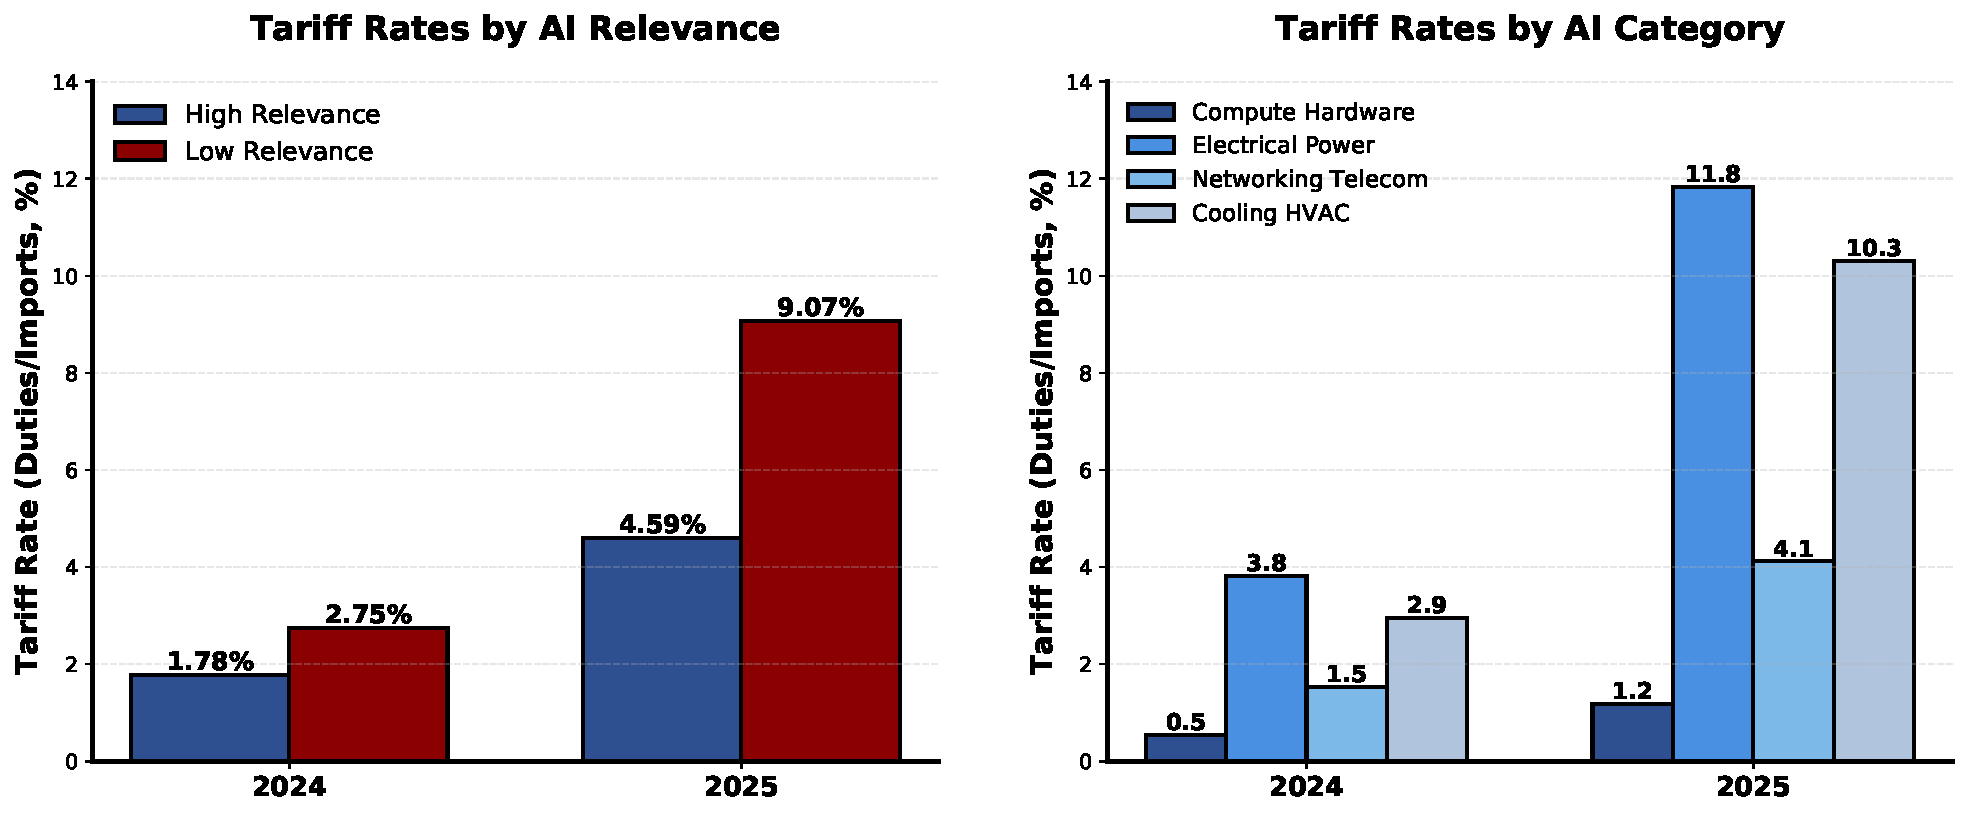
\includegraphics[height=0.55\textheight]{./figures/ai-tariffs.pdf}
%\end{figure}
%\end{landscape}}





%
%\afterpage{%
%\clearpage
%\begin{landscape}
%\input{table-sector.tex}
%\end{landscape}
%}

\newpage

\bibliography{us-tariff-bibtex}


\newpage

\section{Appendix}\label{appendix}

\begin{prompt}
\noindent

\textbf{System Prompt:}

\medskip

You are an expert in AI data center construction, operations, and supply chains. Your task is to classify products by their relevance to building and operating AI-focused data centers (hyperscale facilities running GPU clusters for training and inference. You will be provided with two pieces of information about each product:\\

1. **HS10 Code and Description**: The Harmonized System (HS) is an international product classification used for trade statistics. The HS10 code is a 10-digit code used by U.S. Customs to classify imported goods. The description tells you what the physical product is.\\

2. **NAICS Code and Description**: The North American Industry Classification System (NAICS) indicates which U.S. industry produces or uses this product. This provides additional context about the product's typical industrial application.\\

Consider these categories of relevant products: COMPUTE: GPUs, CPUs, memory, PCBs, servers, storage drives, semiconductors; NETWORKING: Fiber optics, switches, routers, transceivers, cables; COOLING: Chillers, cooling towers, CRAH units, fans, pumps, refrigerants; ELECTRICAL: Transformers, switchgear, UPS, batteries, generators, cables; BUILDING: Structural steel, concrete, rebar, insulation, raised floors; SPECIALTY MATERIALS: Rare earths, copper, aluminum, tantalum, thermal interface materials...).

\medskip

Consider these categories of relevant products:

\begin{itemize}
    \item \textbf{COMPUTE:} GPUs, CPUs, memory, PCBs, servers, storage drives, semiconductors
    \item \textbf{NETWORKING:} Fiber optics, switches, routers, transceivers, cables
    \item \textbf{COOLING:} Chillers, cooling towers, CRAH units, fans, pumps, refrigerants, glycol
    \item \textbf{ELECTRICAL:} Transformers, switchgear, UPS, batteries, generators, cables, busbars
    \item \textbf{BUILDING:} Structural steel, concrete, rebar, insulation, raised floors, fire suppression
    \item \textbf{SPECIALTY MATERIALS:} Rare earths, copper, aluminum, tantalum, thermal interface materials
\end{itemize}

\medskip

Be thoughtful about edge cases:
\begin{itemize}
    \item ``Diesel engines'' could be for generators (relevant) or vehicles (not relevant)
    \item ``Pumps'' could be for cooling systems (relevant) or unrelated industrial use
    \item ``Copper wire'' is relevant for electrical systems
    \item Food, textiles, furniture, and consumer goods are generally NOT relevant
\end{itemize}

\medskip

Use the \texttt{classify\_hs10\_code} tool to record your assessment.

\bigskip
\hrule
\bigskip

\textbf{User Prompt:}

\medskip

Classify this HS10 code:

Code: \{hs10\_code\}

Description: \{description\}

\bigskip
\hrule
\bigskip

\textbf{Tool Schema (Structured Output):}

\medskip

\texttt{relevance}: enum [``High'', ``Medium'', ``Low'']

\texttt{confidence}: integer, 0--100

\texttt{primary\_category}: enum [``Compute\_Hardware'', ``Networking\_Telecom'', ``Cooling\_HVAC'', ``Electrical\_Power'', ``Building\_Structure'', ``Fire\_Safety\_Security'', ``Specialty\_Materials'', ``Maintenance\_Operations'', ``Not\_DC\_Related'']

\texttt{specific\_use}: string (e.g., ``GPU accelerators'', ``backup generator fuel'')

\texttt{reasoning}: string (explanation of classification decision)

\end{prompt}

\newpage

\afterpage{%
\clearpage
\begin{landscape}
\begin{table}[htbp]
\centering
\footnotesize
\caption{Top 10 HS10 Codes by 2025 Import Volume with High AI Relevance}
\label{tab:top10_high_relevance_landscape}
\setlength{\tabcolsep}{2mm}
\renewcommand{\arraystretch}{1.0}
\begin{tabular}{lp{4cm}lp{6cm}ccc}
\toprule
HS10 Code & Description & Category & LLM Reasoning & 2025 Imports (\$B) & Share (\%) & Change (\%) \\
\midrule
8471500150 & {\scriptsize PROC UNT IN HOUS W/ EITHER STOR, IN\&OUTPUT,W/O CRT} & Compute Hardware & {\scriptsize Digital processing units are core compute hardware essential for AI data centers.} & 122.36 & 23.80 & +231.4 \\
8517620090 & {\scriptsize MACH FOR RECP/CONVER ETC OF VOICE/IMAGE/DATA NESOI} & Networking Telecom & {\scriptsize This HS code covers telecommunication equipment for data transmission and conversion, which is essential for AI data centers.} & 42.29 & 8.23 & +26.6 \\
8473301180 & {\scriptsize PTS ADP MCH, NT INCPTNG CRT,PRT CRT ASSEM.;NESOI} & Compute Hardware & {\scriptsize This code covers parts and accessories for automatic data processing machines, specifically including printed circuit assemblies.} & 39.79 & 7.74 & +144.0 \\
8517620020 & {\scriptsize SWITCHING AND ROUTING APPARATUS} & Networking Telecom & {\scriptsize Switching and routing apparatus are core networking components essential for AI data centers.} & 23.80 & 4.63 & +46.4 \\
8473301140 & {\scriptsize PTS ADP MCH, NT INCPTG CRT,PRT CT ASM.,MRY MODULES} & Compute Hardware & {\scriptsize This code covers critical components for data processing machines including memory modules and printed circuit assemblies, which are essential components in AI data center servers, GPU systems, and compute infrastructure.} & 19.26 & 3.75 & +128.4 \\
7403110000 & {\scriptsize REFINED COPPER CATHODES AND SECTIONS OF CATHODES} & Specialty Materials & {\scriptsize Refined copper cathodes are the primary raw material for manufacturing copper products used extensively in data centers.} & 13.88 & 2.70 & +108.9 \\
8523510000 & {\scriptsize SOLID-STATE NON-VOLATILE STORAGE DEVICES} & Compute Hardware & {\scriptsize Solid-state non-volatile storage devices are essential components in AI data centers, used as high-performance storage drives in servers, storage arrays, and compute nodes.} & 13.73 & 2.67 & +44.5 \\
8507600020 & {\scriptsize LITHIUM-ION STORAGE BATTERIES, NESOI} & Electrical Power & {\scriptsize Lithium-ion storage batteries are critical components in data center UPS (Uninterruptible Power Supply) systems, providing backup power during outages and power conditioning.} & 13.69 & 2.66 & -8.0 \\
8471804000 & {\scriptsize UNITS,NESOI,FOR INCORPORATION INTO ADP MACHINES} & Compute Hardware & {\scriptsize This HS code covers units designed for physical incorporation into automatic data processing machines, which directly includes server components, processing modules, and other compute hardware essential for AI data center operations.} & 10.17 & 1.98 & +846.3 \\
8537109170 & {\scriptsize ELECTRICL APP EQP W/ APPS FM 8535\&6,LT 1000V,NESOI} & Electrical Power & {\scriptsize This code covers electrical control and distribution bases/panels for voltages up to 1,000V, which are essential components in data center electrical infrastructure.} & 9.41 & 1.83 & -6.1 \\
\bottomrule
\end{tabular}
\end{table}
\end{landscape}

}


\newpage

\afterpage{%
\clearpage
\begin{landscape}
\begin{table}[htbp]
\centering
\footnotesize
\caption{HS10 Codes Ranked 11-20 by 2025 Import Volume with High AI Relevance}
\label{tab:top11to20_high_relevance_landscape}
\setlength{\tabcolsep}{2mm}
\renewcommand{\arraystretch}{1.0}
\begin{tabular}{lp{4cm}lp{6cm}ccc}
\toprule
HS10 Code & Description & Category & LLM Reasoning & 2025 Imports (\$B) & Share (\%) & Change (\%) \\
\midrule
8542310045 & {\scriptsize PRCSSRS (INCL MICRO): CENTRL PROCSSNG UNITS (CPUS)} & Compute Hardware & {\scriptsize CPUs are essential compute hardware in AI data centers, serving as host processors in GPU-accelerated servers, handling system management, I/O operations, and coordination tasks in AI training and inference workloads} & 10.28 & 1.60 & +0.0 \\
8471704065 & {\scriptsize HARD DISK DRIVE UNT, NESOI, W/OUT EXTNL POWR SUPLY} & Compute Hardware & {\scriptsize Hard disk drives are essential storage components in AI data centers, used in servers for data storage, backup systems, and distributed storage arrays that support AI training datasets and model storage} & 6.72 & 1.05 & +68.3 \\
8542310050 & {\scriptsize PROCESSORS (INCLUDING MICROPROCESSORS): OTHER} & Compute Hardware & {\scriptsize Processors and microprocessors are core compute components essential for AI data centers.} & 6.66 & 1.04 & +0.0 \\
8473305100 & {\scriptsize PTS \& ACCESSORIES OF MACH OF HEADING OF 8471,NESOI} & Compute Hardware & {\scriptsize This code covers parts and accessories for machines of heading 8471 (automatic data processing machines/computers).} & 5.52 & 0.86 & +66.2 \\
8544429090 & {\scriptsize INSULATD ELEC CONDCTR LT=1000V,W/ CONNECTRS, NESOI} & Electrical Power & {\scriptsize Insulated electric conductors with connectors for voltages up to 1000V are essential for data center electrical infrastructure.} & 4.85 & 0.75 & +17.4 \\
8471709000 & {\scriptsize OTHER STORAGE UNITS, NESOI} & Compute Hardware & {\scriptsize This HS code covers storage units not elsewhere specified in the 8471 category (automatic data processing machines).} & 4.24 & 0.66 & +136.3 \\
8542310075 & {\scriptsize PROCESSORS \& CONTOLLERS W/NOT COMBO W MEMORIS, ETC} & Compute Hardware & {\scriptsize This code covers processors and controllers which are core computing components in AI data centers.} & 4.14 & 0.64 & +0.0 \\
8537109160 & {\scriptsize PROGRAMABLE CONTROLLERS, LT=1,000 VOLTS} & Electrical Power & {\scriptsize Programmable controllers (PLCs) are essential for data center operations, controlling HVAC systems, power distribution, lighting, security systems, and coordinating various building automation functions.} & 4.14 & 0.64 & +9.1 \\
8486900000 & {\scriptsize PARTS \& ACCESSORIES FOR MACH/APPS OF HDG 8486} & Compute Hardware & {\scriptsize This equipment is essential for manufacturing semiconductors, electronic integrated circuits, and related components that are fundamental to AI data center hardware including GPUs, CPUs, memory modules, and other critical compute infrastructure} & 3.87 & 0.60 & +13.5 \\
8544700000 & {\scriptsize INSULATED OPTICAL FIBER CABLES WITH INDVULY SH FBR} & Networking Telecom & {\scriptsize Optical fiber cables are critical infrastructure for AI data centers, enabling high-bandwidth, low-latency communication required for GPU clusters, distributed training, and inter-rack networking.} & 3.84 & 0.60 & +68.9 \\
\bottomrule
\end{tabular}
\end{table}
\end{landscape}

}



\end{onehalfspacing}

\end{document}
